\section{Modo Protegido}

\subsection{Selector de Segmento}
Al entrar a modo protegido, inicializamos los diferentes selectores de segmento. Los mismos tienen el siguiente formato:

\begin{figure}[h!]
  \centering
    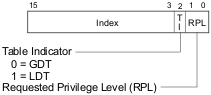
\includegraphics[scale=0.8]{segment_selector}
  \caption{Segment Selector}
\end{figure}

\subsection{Niveles de protección}

Intel soporta 4 niveles de protección diferentes, siendo 0 el mas alto y 4 el mas bajo. Por esa razón los bits de protección tienen 2 bits.

\begin{figure}[h!]
  \centering
    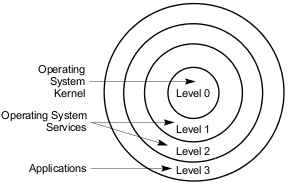
\includegraphics[width=0.4\textwidth]{protection_rings}
  \caption{IDT Descriptor}
\end{figure}

TODO: Escribir un poco como funciona la unidad de protección con RPL, DPL Y CPL.

\subsection{Interrupt Descriptor Table}

Una interrupción es una señal que le indica a la CPU que debe interrumpir la ejecución actual de instrucciones. El rol de la \texttt{IDT} (Interrupt Descriptor Table) es contener los diferentes descriptores de interrupcion y asociar las diferentes interrupciones a sus respectivas rutinas de atención de interrupción. Existen tres fuentes de interrupciones:

\begin{enumerate}
\item Hardware
\item Software
\item Internas
\end{enumerate}

A su vez, la \texttt{IDT} puede contener tres tipos de descriptores:

\begin{enumerate}
\item Interrupt Gate
\item Trap Gate
\item Task Gate
\end{enumerate}

Para construir la IDT, armamos primero en C la estructura \texttt{idt\_entry} con sus respectivos atributos y luego construimos un array de 256 posiciones del mismo (la máxima cantidad soportada por el procesador). En este trabajo practico solo utilizaremos descriptores de interrupción y de tarea.

\begin{figure}[h!]
  \centering
    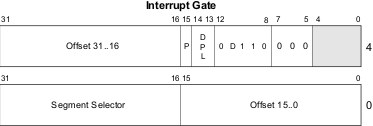
\includegraphics[width=0.5\textwidth]{idt_desc}
  \caption{IDT Descriptor}
\end{figure}

 Modificamos la macro de la cátedra para poder cargar la IDT con diferentes atributos. Luego inicializamos las diferentes posiciones que utilizamos con sus respectivos selectores de segmento y atributos, tomando también la referencia a las respectivas rutinas de atención.

Hay que tener mucho cuidado al settear los atributos. Caso contrario, al cambiar de segmento podemos tener un General Protection Fault (\#GP). Algunos atributos son:

\begin{enumerate}
\item P: Present flag. 1 if present.
\item DPL: Descriptor Protection Level. Nivel de privilegios del descriptor.
\item D: Size of gate. 1 = 32 bits; 0 = 16 bits.
\end{enumerate}

Un procesador Intel reserva por default las primeras 31 posiciones de la \texttt{IDT} para las diferentes excepciones del procesador. Actualmente, el procesador solo utiliza las primeras 21. Inicializamos estas excepciones del procesador a una rutina que imprime la excepción en pantalla.

Mas adelante inicializaremos otros descriptores de la \texttt{IDT} para atender otras interrupciones como la del reloj y la del teclado.

Una vez cargada la IDT, se debe remapear el PIC (Programmable Interrupt Controler) para referir a las nuevas interrupciones que agreguemos. Esto se hace con las rutinas de la catedra \texttt{resetear\_pic} y luego \texttt{habilitar\_pic}.

\subsection{Memory Management Unit}
Un procesador Intel, para gestionar lo que son los accesos a memoria, utiliza una \texttt{MMU} (Memory Management Unit). La misma esta compuesta por la Unidad de Segmentación y la Unidad de Paginación.

\begin{figure}[H]
  \centering
    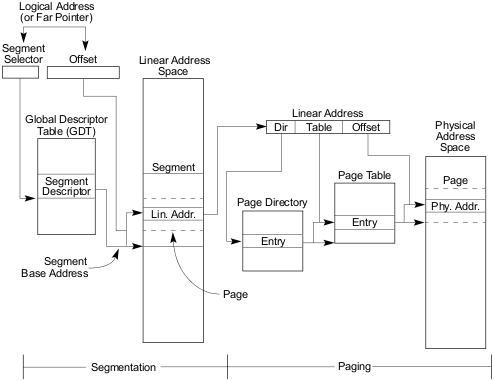
\includegraphics[width=0.6\textwidth]{memory_management}
  \caption{Segmentation \& Paging}
\end{figure}

La paginacion nos permite que cada tarea pueda tener su propia \texttt{memoria virtual}, mappeando direcciones físicas a direcciones virtuales.

\subsubsection{Unidad de Segmentación}

La unidad de segmentación se ocupa de pasar desde las \textit{direcciones lógicas} a direcciones lineales. Para ello, utiliza la GDT para identificar el segmento adecuado y luego su respectivo offset. La unidad de protección verifica que el \texttt{RPL} es compatible con el \texttt{CPL} y el \texttt{DPL}.

En modo protegido, los selectores de segmento tienen 16 bits. Los 13 bits mas significativos contienen el indice dentro de la tabla de descriptores. El bit 2 especifica si la operación utiliza la \texttt{GDT} o la \texttt{LDT}. Finalmente, los 2 bits menos significativos definen el nivel de privilegio solicitado.

\subsubsection{Unidad de Paginación}

Para activar la paginación, en primer lugar debemos inicializar el directorio de paginas y cargar el registro \reg{cr3} con la dirección del mismo. Como los directorios de paginas estan alineados a 4 kb, los primeros 20 bits del cr3 no son necesarios para identificar el directorio, por lo que son utilizados por atributos del procesador. En nuestro caso no utilizamos estos atributos, por lo que son todos 0.

Luego, debemos activar la paginacion con el ultimo bit del registro \reg{cr0}.

Si la paginación esta activada, la dirección lineal luego pasa por la unidad de paginación. La unidad de paginación se encarga de ir desde la dirección lineal a la dirección física en memoria. En caso de que la dirección lineal no este paginada, el procesador tiene una page fault exception.

Para facilitar el manejo del armado de estructuras para la paginación, se crearon las siguientes funciones en C. Antes de explicar que hace cada función, un comentario. Cada directorio de paginas tiene 1024 entradas de descriptores de 4 bytes. Lo mismo sucede con los directorios de paginas, que también tienen 1024 entradas con descriptores de 4 bytes. El procesador, al buscar estas estructuras en memoria RAM, requiere que las mismas estén alineadas a 4kb, dado que es el tamaño de pagina que carga en memoria cache.

\begin{enumerate}
\item \fun{create\_page\_table(uint directoryBase, uint directoryEntry, uint physicalAddress, uchar readWrite, uchar userSupervisor)}: Asigna una \texttt{page\_table} a una tabla de directorios con los atributos pasados por parametro. Al final de la función, se limpia la memoria cache para garantizar que cuando el procesador busca esta pagina, la misma se encuentra actualizada.

\item \fun{delete\_page\_table(uint directoryBase, uint directoryEntry)}: Borra una tabla de paginas de un directorio de paginas. Esto lo hace simplemente setteando el bit P (present) en cada pagina en 0.

\item \fun{create\_page(uint directoryBase, uint directoryEntry, uint tableEntry, uint physicalAddress, \\ uchar readWrite, uchar userSupervisor)}: Crea una pagina en la tabla de paginas de algún directorio.

\item \fun{delete\_page(uint directoryBase, uint directoryEntry, uint tableEntry)}: Borra una pagina en la tabla de paginas de algún directorio. Esto lo hace setteando el bit P en 0.

\item \fun{mmap(uint virtualAddress, uint physicalAddress, uint directoryBase, uchar readWrite, \\ uchar userSupervisor)}: Mappea una dirección virtual en una direccion fisica. Para esto, primero se busca la tabla de paginas y la pagina correspondiente a la dirección virtual. Luego se le asigna a esa pagina la dirección física. Esto se hace de la siguiente forma:
	\begin{enumerate}
	\item A partir de la dirección virtual, se busca la entrada de directorio correspondiente a la misma. Esto se hace dividiendo el virtualAdress por el tamaño direccionable por cada page\_directory.$virtualAdress / 1024*4kb$. Esto es equivalente a $virtualAdress >> 22$.
	\item Buscamos el indice en la entrada de paginas. Esto se calcula dividiendo por el tamaño de pagina e ignorando los bits correspondientes a la entrada de directorio $virtualAdress / 4kb$ $\&$ $0x3FF$, que es equivalente a $virtualAdress >> 12$ $\&$ $0x3FF$.
	\end{enumerate}

\item \fun{munmap(uint directoryBase, uint virtualAddress)}: Desmappea la pagina correspondiente a una dirección virtual. Calcula todos los indices necesarios de la misma manera que \fun{mmap}

\item \fun{mmu\_inicializar\_dir\_kernel()}: Inicializa el directorio del kernel. Para ello, hacemos memory mapping sobre el kernel y le asignamos un area libre, todo desde \addr{0x00000000} a \addr{0x003FFFF}.

\item \fun{mmu\_inicializar\_dir\_pirata(uint directoryBase, uint pirateCodeBaseSrc, uint pirateCodeBaseDst)}: Esta función inicializa el directorio de un pirata. Al igual que el Kernel, hacemos memory mapping, aunque en modo user y en read only. A su vez, mappeamos la pagina donde vamos a poner el codigo del pirata, y copiamos el código del pirata que se encuentra en el Kernel en esta pagina.

\item \fun{mmu\_move\_codepage(uint src, uint dst, pirata\_t *p)}: Mueve la pagina de codigo del pirata desde $src$ a $dst$.

No implementamos la funcion \texttt{mmu\_inicializar} dado que todo el trabajo lo hace \texttt{mmu\_inicializar\_dir\_kernel}.

\end{enumerate}

\subsection{Otras Interrupciones}

Para inicializar otras interrupciones, tenemos que agregar los diferentes descriptores a la IDT, que apuntan a su correspondiente rutina de atención y ademas tienen los atributos correctos. Recordemos que las rutinas de atención de la interrupción deben ser transparentes a lo que el procesador estaba ejecutando en el momento, por lo que se debe guardar todos los registros y luego restaurarlos al finalizar la rutina de atención. Ademas, las interrupciones en general llevan a un escalamiento de privilegios, por lo que los privilegios también deben ser restaurados.

A su vez, la rutina de atención de la interrupción debe indicarle al pic que la interrupción esta siendo atendida, para que otras interrupciones puedan suceder. Esto se hace con la función de la cátedra \fun{fin\_intr\_pic1}.

\subsubsection{Reloj}

Esta es una interrupción interna, que sucede con cada \texttt{tick} del reloj del procesador. La rutina de atención de esta interrupción se encarga de mostrar la animación de un cursor rotando en la esquina inferior derecha de la pantalla, por medio de la función \fun{screen\_actualizar\_reloj\_global}.

\subsubsection{Teclado}
Utilizaremos la rutina de atención del teclado para habilitar las diferentes teclas disponibles a los jugadores. Cuando programábamos esto, notamos que es necesario tomar la tecla presionada desde el controlador del teclado, caso contrario el teclado no vuelve a solicitar una interrupción.

\subsubsection{Software}
Asignamos a la interrupción \addr{0x46} (70) una rutina que atiende un servicio del sistema.

\subsection{Task State Segment}

La \texttt{TSS} (Task State Segment) es el espacio de memoria previsto en los procesadores \texttt{IA-32} como el espacio de contexto de cada tarea. Este segmento debe tener su respectivo descriptor en la \texttt{GDT}. Ademas, el selector de segmento de la tarea que se
esta ejecutando actualmente se debe encontrar en el registro \reg{TR} (Task Register).

Para llamar a una tarea, se lleva a cabo un \texttt{call far} con su respectivo selector de segmento. Si ya estabamos ejecutando una tarea, se guarda su contexto en \reg{TR} antes de ejecutar la nueva tarea. 

La primera vez que llamamos a una tarea, el registro \reg{TR} no tiene un valor definido. Ademas, debemos guardar el contexto del programa en ejecucion. Para ello, se crea una tarea inicial  en la \texttt{TSS} para que el procesador tenga donde guardar el contexto actual.

\subsection{Scheduler}